\documentclass[11pt,letterpaper]{article}

\usepackage[utf8]{inputenc}
\usepackage[T1]{fontenc}
\usepackage[spanish,es-nodecimaldot,es-tabla,es-noshorthands]{babel}
\usepackage{lmodern}
\usepackage[margin=2.3cm]{geometry}
\usepackage{graphicx}
\usepackage{booktabs}
\usepackage{tabularx}
\usepackage{array}
\usepackage{amsmath,amssymb}
\usepackage{xcolor}
\usepackage{tikz}
\usetikzlibrary{arrows.meta,positioning,shapes.geometric}
\usepackage{caption}
\usepackage{float}
\usepackage{enumitem}
\usepackage[hidelinks]{hyperref}

\graphicspath{{../docs/}}
\setlist{itemsep=2pt,topsep=4pt}
\captionsetup{font=small,labelfont=bf}
\newcolumntype{Y}{>{\raggedright\arraybackslash}X}

\title{\textbf{FacturaSegura: detección de facturas alteradas\\en reembolsos de gastos con redes convolucionales}\\[4pt]
\large Proyecto final --- CC3092 Deep Learning y Sistemas Inteligentes}
\author{Isabella Obando Guzmán (23074) \and Anthony Lou Schwank (CARNÉ)}
\date{18 de noviembre de 2026}

\begin{document}
\maketitle

\begin{abstract}
Las empresas reembolsan gastos a partir de la foto de una factura, y editar esa foto en el celular para subir el total, cambiar la fecha o poner el NIT de la empresa en una compra personal toma un minuto. \textbf{FacturaSegura} es un detector de facturas alteradas basado en una red convolucional (EfficientNet-B0 preentrenada en ImageNet y ajustada por el grupo, sin LLMs). Estima la probabilidad de que la foto haya sido editada y marca la zona sospechosa, y solo las facturas que superan un umbral elegido según el valor de negocio van a auditoría. Se entrenó con un generador propio de facturas FEL guatemaltecas fotografiadas, cada una con una gemela alterada alineada píxel a píxel. En el conjunto de prueba sintético, el modelo final alcanza AUC 0.981, detecta el 93\,\% de las alteraciones con 1\,\% de falsas alarmas y localiza la zona editada en el 87\,\% de los casos. Con una prevalencia supuesta de 3\,\% de facturas alteradas, genera un ahorro neto de \textbf{Q9,162 por cada 1,000 facturas}: detiene el 94\,\% del fraude, frente a $-$Q19,107 de auditar todas y $-$Q77 de reglas fiscales con lectura perfecta. Las iteraciones muestran que mejorar la métrica técnica no siempre aumenta el valor y que el modelo está cerca del techo de ahorro posible. Todos los resultados son sintéticos; la validación con fotos reales queda pendiente.
\end{abstract}

\section{Contexto de negocio y definición del problema}

\paragraph{Quién se beneficia.} Empresas medianas y grandes en Guatemala que reembolsan gastos a sus empleados (viáticos, combustible, comidas, compras menores). El empleado envía la foto de la factura (por correo, WhatsApp o una app interna) y el área de contabilidad la aprueba o la rechaza. Desde la adopción de la Factura Electrónica en Línea (FEL) de la SAT, la mayoría de comprobantes son tickets térmicos o representaciones impresas de documentos electrónicos, y quien los recibe solo tiene la imagen.

\paragraph{Cómo se resuelve hoy y cuánto cuesta.} Hay dos extremos. \emph{No revisar} sale gratis en auditoría, pero deja pasar todo el fraude. \emph{Revisar todo} detiene el fraude, pero cuesta el tiempo de un auditor por factura y genera fricción con los empleados honestos. Con los supuestos de la sección~\ref{sec:valor} (3\,\% de facturas alteradas, Q10 por auditoría, Q20 de fricción por sospechar de un empleado honesto), por cada 1,000 facturas:
\begin{itemize}
  \item No revisar nada pierde \textbf{Q10,293} de fraude (línea base de pérdida).
  \item Auditar todas cuesta más de lo que evita: valor neto de \textbf{$-$Q19,107}.
\end{itemize}

\paragraph{Por qué deep learning.} Una alteración hecha con una app deja huellas visuales pequeñas: un parche de color plano, una fuente o un grosor de trazo que no calza, un texto sin la inclinación de la foto, o un borde donde se pegó un dígito. En nuestros datos, la zona editada ocupa en mediana el \textbf{0.25\,\%} de la foto. Detectarlas requiere aprender patrones locales de textura y tipografía, que es justo lo que hacen bien las redes convolucionales. Se evaluaron dos alternativas más simples (sección~\ref{sec:resultados}):
\begin{itemize}
  \item \textbf{Reglas fiscales FEL} (IVA = 12/112 del total, dígito verificador del NIT, coherencia entre serie, número y autorización), aplicadas a los valores visibles suponiendo un OCR perfecto. Detectan el 47\,\% con 14\,\% de falsas alarmas.
  \item \textbf{Error Level Analysis (ELA)}, una técnica forense clásica. Da AUC 0.51 (azar), porque la recompresión tipo WhatsApp borra su señal.
\end{itemize}
Ninguna de las dos genera ahorro positivo, y eso justifica la complejidad de una CNN.

\paragraph{KPIs de negocio.} Los indicadores son el fraude detenido (Q), el costo de auditoría (facturas auditadas $\times$ costo), la fricción con empleados honestos (falsas alarmas $\times$ costo) y el \textbf{valor neto por cada 1,000 facturas}, que los resume. La línea base es no revisar nada (valor 0 y Q10,293 de fraude perdido).

\section{Datos y análisis exploratorio}
\label{sec:datos}

\paragraph{Fuente.} No existe un dataset público de facturas guatemaltecas alteradas, y juntar miles de fotos reales con su versión editada no es viable en el tiempo del proyecto. Por eso se construyó un \textbf{generador sintético} (\texttt{src/synth\_fel.py}, extendido de un proyecto anterior del curso), que produce facturas FEL ficticias pero internamente consistentes: NIT con dígito verificador módulo 11, serie y número derivados del número de autorización, IVA de 12/112 o IDP en gasolineras. Las facturas son tickets térmicos o facturas tamaño carta de seis tipos de comercio. Cada documento se ``fotografía'' con perspectiva, rotación, fondo, sombras, papel desteñido, arrugas, desenfoque, ruido y compresión JPEG. El generador registra la posición de cada campo y la homografía documento$\to$foto, lo que permite alterar campos concretos en la foto final.

\paragraph{Alteraciones.} Sobre la foto final (como en un fraude real: se toma la foto y luego se edita), \texttt{src/tamper.py} aplica dos técnicas:
\begin{itemize}
  \item \textbf{Reescribir:} se tapa el valor con el color del papel y se escribe otro encima.
  \item \textbf{Copiar un dígito:} se toma un dígito de otra parte de la misma factura y se pega sobre otro.
\end{itemize}
Cada alteración tiene un nivel de dificultad:
\begin{itemize}
  \item \textbf{Fácil:} otra fuente, texto horizontal y parche liso, lo típico de una app.
  \item \textbf{Media:} la misma fuente, rotación y tinta.
  \item \textbf{Difícil:} además imita el ruido y el desenfoque, o copia un dígito de la misma factura.
\end{itemize}
Las alteraciones siempre son fraudes plausibles: los montos solo suben, las fechas cambian solo día o mes y existen, y el NIT nuevo es válido. Cada una guarda su \textbf{máscara} y su \textbf{monto en riesgo}, es decir, lo que gana quien altera. Ese monto es la diferencia inflada si se cambia el total o el IVA, y el total completo si se cambia la fecha (reutilizar una factura vieja) o el NIT del comprador (cobrar una compra personal). La figura~\ref{fig:alteraciones} muestra ejemplos.

\paragraph{Pares alineados.} Por cada factura se guardan dos versiones de la \emph{misma} foto: la auténtica y la alterada. Ambas pasan por el mismo post-proceso (recorte, brillo y reescalado idénticos, con recompresión JPEG independiente), de modo que quedan alineadas píxel a píxel. Fuera de la zona editada solo difieren por ruido de compresión (2--5 niveles de gris en promedio).

\begin{figure}[t]
  \centering
  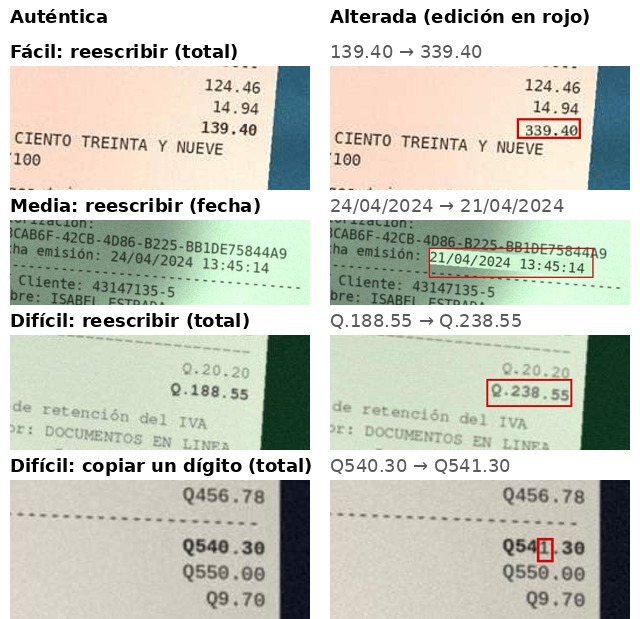
\includegraphics[width=0.62\textwidth]{ejemplos_alteraciones.jpg}
  \caption{Ejemplos del conjunto de prueba: foto auténtica (izquierda) y su gemela alterada (derecha), por nivel de dificultad. Las alteraciones difíciles son casi imperceptibles para una persona.}
  \label{fig:alteraciones}
\end{figure}

\paragraph{Volumen y formato.} Las fotos son JPEG de hasta 1600 px por lado (300--1472 px de ancho y 570--1600 de alto) con su máscara PNG y metadatos en JSONL. Los conjuntos son:
\begin{itemize}
  \item 3,000 pares de entrenamiento, 300 de validación y 300 de prueba;
  \item un lote extra de 3,000 pares con más casos difíciles, usado desde la iteración 4.
\end{itemize}
Las clases están balanceadas (50/50) en todos los conjuntos. La prevalencia real supuesta (3\,\%) se introduce en el modelo de valor, no en el entrenamiento.

\paragraph{Análisis exploratorio.} En el conjunto de entrenamiento base:
\begin{itemize}
  \item \textbf{Formatos:} 76\,\% tickets y 24\,\% facturas carta.
  \item \textbf{Comercios:} seis tipos, con unas 500 facturas cada uno.
  \item \textbf{Campos alterados:} total 57\,\%, NIT del receptor 15\,\%, fecha 12\,\%, productos 6\,\%, NIT del emisor 5\,\% e IVA 4\,\%.
  \item \textbf{Dificultad:} 50\,\% fácil, 31\,\% media y 19\,\% difícil (1,502 / 920 / 578).
  \item \textbf{Monto en riesgo:} media Q337, mediana Q181, percentil 90 de Q700 y máximo Q8,000. La distribución está sesgada a la derecha, y 6\,\% de las alteraciones (productos sin cambio del total) no tienen ganancia.
  \item \textbf{Facturas:} el total tiene media de Q364 y mediana de Q231.
  \item \textbf{Tamaño de la zona editada:} mediana de 0.25\,\% y percentil 90 de 0.51\,\% de la foto. Este dato motivó la arquitectura (sección~\ref{sec:metodo}).
  \item \textbf{Calidad de los datos:} no hay valores nulos ni etiquetas ruidosas, porque la verdad es exacta por construcción.
\end{itemize}
El sesgo principal es de \emph{representatividad}: las fuentes, diseños de ticket y técnicas de edición son las que el generador sabe imitar.

\paragraph{División y fugas.} Cada conjunto usa una semilla distinta, y las dos versiones de un par siempre van al mismo conjunto, para que el modelo no vea en entrenamiento la gemela de una foto de prueba. La generación es determinista por semilla, lo cual se verifica con pruebas automáticas. El umbral de operación se elige en validación y la prueba solo se usa para reportar.

\paragraph{Privacidad y licencias.} Los datos sintéticos no contienen información de personas ni comercios reales. Las fuentes incluidas son libres (DejaVu, Liberation, FreeFont y Go, con sus licencias en \texttt{src/fonts}). Las fotos reales de prueba que se recolecten pueden incluir NIT y nombres, así que se mantienen fuera del repositorio.

\section{Modelo de valor}
\label{sec:valor}

Por cada 1,000 facturas de reembolso y un umbral $t$ sobre la probabilidad $p$ de alteración:
\begin{align*}
\text{valor}(t) ={} & \underbrace{1000\,\pi\;\mathbb{E}\big[M\cdot\mathbf{1}(p\ge t)\mid\text{alterada}\big]}_{\text{fraude detenido}}\\
 & -\underbrace{1000\,\big(\pi\,\mathrm{TPR}(t)+(1-\pi)\,\mathrm{FPR}(t)\big)\,c_{\text{rev}}}_{\text{costo de auditar las facturas marcadas}}
   -\underbrace{1000\,(1-\pi)\,\mathrm{FPR}(t)\,c_{\text{fric}}}_{\text{fricción con empleados honestos}}
\end{align*}
donde $\pi$ es la prevalencia de facturas alteradas y $M$ el monto en riesgo. El valor de ``no revisar nada'' es 0, y el de ``auditar todo'' es el caso $t=0$.

\paragraph{Supuestos y fuentes.} Todos los parámetros son estimaciones razonables, no mediciones, y por eso se someten a análisis de sensibilidad:
\begin{itemize}
  \item \textbf{$\pi = 3$\,\% de facturas alteradas.} No hay estadística pública para Guatemala; los reembolsos de gastos son uno de los esquemas de fraude ocupacional más frecuentes. Es el supuesto más incierto.
  \item \textbf{$c_{\text{rev}}$ = Q10 por auditoría:} unos 10 minutos de un auditor o contador a ${\sim}$Q60/hora.
  \item \textbf{$c_{\text{fric}}$ = Q20 por falsa alarma:} tiempo del empleado para justificarse, retraso del reembolso y deterioro de la confianza.
  \item \textbf{$M$:} se toma del monto en riesgo de cada alteración del conjunto de prueba (media Q343). Así, que un fraude de Q1,000 se escape pesa más que uno de Q5.
\end{itemize}
El valor se calcula con las tasas medidas en el conjunto de prueba. El umbral se elige maximizando el valor en \emph{validación} y luego se aplica a prueba.

\paragraph{Curva de valor y punto de operación.} La figura~\ref{fig:valor} muestra el valor en función del umbral para el modelo final. El óptimo elegido en validación es $t=0.88$. En prueba, ese umbral manda a auditoría 34 de cada 1,000 facturas y detiene Q9,631 de los Q10,293 de fraude (94\,\%). El costo es Q340 de auditoría y Q129 de fricción (0.7\,\% de las auténticas), para un \textbf{valor neto de Q9,162}. La curva es plana: cualquier umbral entre 0.43 y 0.99 da más de Q8,500. Lo que destruye valor son los extremos, y auditar todo ($t=0$) pierde Q19,107.

\begin{figure}[t]
  \centering
  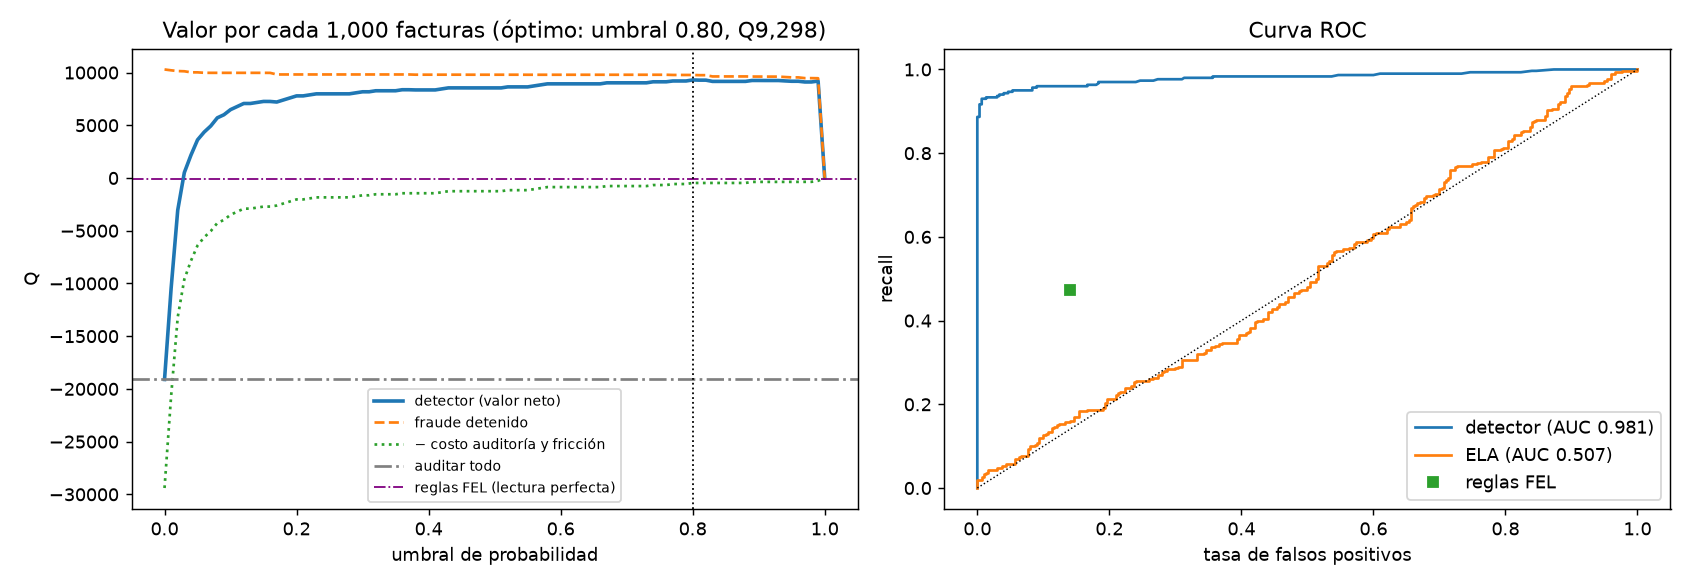
\includegraphics[width=\textwidth]{curva_valor_it5_menos_falsas.png}
  \caption{Izquierda: valor neto por cada 1,000 facturas según el umbral (modelo final), con sus componentes y las líneas base. Derecha: curva ROC del detector frente a ELA y al punto de operación de las reglas FEL.}
  \label{fig:valor}
\end{figure}

\paragraph{Análisis de sensibilidad.} En la tabla~\ref{tab:sens}, en cada escenario se vuelve a elegir el umbral en validación y se reporta el valor en prueba.
\begin{itemize}
  \item \textbf{El valor escala casi proporcionalmente con la prevalencia.} Es el parámetro que una empresa tendría que estimar primero con sus propios datos.
  \item \textbf{Auditar todo} solo conviene si más del ${\sim}$8\,\% de las facturas fueran alteradas.
  \item \textbf{El umbral se adapta como se espera:} más bajo con más fraude y más alto con menos.
  \item \textbf{Un resultado contraintuitivo:} con fricción $-$50\,\%, validación elige un umbral más bajo que en prueba deja pasar más falsas alarmas. Refleja el ruido de elegir umbrales con 300 facturas por clase.
\end{itemize}

\begin{table}[t]
  \centering\small\setlength{\tabcolsep}{4pt}
  \begin{tabular}{lccc}
    \toprule
    Escenario & Umbral (validación) & Valor en prueba (Q/1,000) & Auditar todo \\
    \midrule
    Base ($\pi=3$\,\%, Q10, Q20) & 0.88 & \textbf{9,162} & $-$19,107 \\
    Prevalencia 1\,\% & 0.96 & 2,991 & $-$26,369 \\
    Prevalencia 5\,\% & 0.46 & 14,907 & $-$11,845 \\
    Prevalencia 10\,\% & 0.46 & 30,814 & +6,310 \\
    Costo de auditoría $-$50\,\% / +50\,\% & 0.88 & 9,332 / 8,992 & $-$14,107 / $-$24,107 \\
    Fricción $-$50\,\% / +50\,\% & 0.46 / 0.88 & 8,868 / 9,097 & $-$9,407 / $-$28,807 \\
    \bottomrule
  \end{tabular}
  \caption{Sensibilidad del valor del modelo final a los supuestos.}
  \label{tab:sens}
\end{table}

\section{Metodología de desarrollo}
\label{sec:metodo}

\paragraph{Arquitecturas consideradas.} Todas usan como base \textbf{EfficientNet-B0} (\texttt{timm}, preentrenada en ImageNet, 4.1\,M parámetros). Se eligió por su buena relación precisión/costo y porque permite inferencia en CPU. Se compararon dos cabezas:
\begin{enumerate}
  \item \textbf{Clasificador estándar:} promedio global de la última etapa y capa lineal. Es lo visto en clase para clasificación de imágenes.
  \item \textbf{Mapa de sospecha:} se fusionan las características de stride 16 y 32 (convolución $3\times3$ + BN + SiLU + convolución $1\times1$) en un mapa de logits a 1/16 de la resolución, y la factura se clasifica con el promedio de las $k=8$ celdas más sospechosas.
\end{enumerate}
La segunda es una forma de \emph{multiple instance learning}. Como la alteración ocupa el 0.25\,\% de la foto, el promedio global la diluye, y el top-$k$ no. Además, la red es totalmente convolucional y produce un mapa de calor que sirve como explicación.

\paragraph{Función de pérdida y alineación con el negocio.} La pérdida es BCE de clasificación más BCE del mapa contra la máscara reducida a 1/16, con peso 1. Una celda cuenta como alterada si tiene al menos 25\,\% de píxeles editados. La supervisión con máscara no busca mejorar el AUC: hace que el modelo marque \emph{dónde} está la edición, que es lo que necesita el auditor para revisar rápido. La alineación con el negocio se hace en dos niveles:
\begin{itemize}
  \item \textbf{Selección del checkpoint} por el recall con $\le$1\,\% de falsas alarmas en validación, en vez de por AUC: refleja que una falsa alarma tiene costo.
  \item \textbf{Elección del umbral} por valor (sección~\ref{sec:valor}).
\end{itemize}
También se probó una pérdida ponderada por el monto en riesgo (iteración 6).

\paragraph{Entrenamiento con recortes de gemelas.} En las iteraciones 1 y 2, la foto completa se reduce a $768\times576$. Desde la iteración 3 se entrena con \textbf{recortes de $512\times512$ a resolución completa}: por cada par se toma la \emph{misma ventana} de la foto auténtica y de su gemela alterada. La única diferencia entre los dos recortes es la edición, así que el modelo no puede usar el estilo de la factura como atajo. En validación y en uso, la red recibe la foto completa (hasta 1600 px, con relleno a múltiplo de 128).

\paragraph{Hiperparámetros y búsqueda.}
\begin{itemize}
  \item \textbf{Optimización:} AdamW (lr máximo $3\times10^{-4}$, weight decay $10^{-4}$) con OneCycle (10\,\% de calentamiento) y recorte del gradiente a norma 2.
  \item \textbf{Lote y épocas:} 8 pares por lote (16 recortes) y 10 épocas.
  \item \textbf{Precisión:} bf16 autocast.
\end{itemize}
La búsqueda fue \emph{guiada por diagnóstico}: un cambio por iteración, decidido a partir del análisis de errores de la anterior, en lugar de una búsqueda en malla. El costo de cada entrenamiento (unos 40 minutos) y la meta de entender qué mueve el valor favorecían ese enfoque.

\paragraph{Uso de modelos preentrenados y costo computacional.} Se hizo fine-tuning completo desde los pesos de ImageNet. Todo se entrenó en una GPU de laptop (RTX 3070, 8\,GB): cada iteración tomó entre 22 y 77 minutos con menos de 4\,GB de VRAM, y el proyecto completo usó unas 5 horas de GPU, con un costo eléctrico despreciable. El modelo final pesa 17\,MB.

\section{Resultados de las iteraciones}
\label{sec:resultados}

\begin{table}[t]
  \centering\small
  \begin{tabularx}{\textwidth}{l Y c c c c c r}
    \toprule
    It. & Cambio respecto a la anterior & AUC & Recall@ & Recall & Locali- & Ahorro & Min. \\
        &                               &     & FPR 1\% & difícil & zación & Q/1,000 & GPU \\
    \midrule
    it1 & EfficientNet-B0, foto reducida $768\times576$, clasificador estándar & 0.950 & 82\% & 59\% & --- & 7,791 & 40 \\
    it2 & + mapa de sospecha, top-8 y máscaras & 0.954 & 87\% & 56\% & 71\% & 8,643 & 39 \\
    it3 & + recortes de 512 a resolución completa & 0.961 & 90\% & 66\% & 80\% & 9,000 & 27 \\
    it3b & ablación: it3 sin máscaras & 0.964 & 90\% & 61\% & 0\% & 9,294 & 22 \\
    it4 & + lote extra con más casos difíciles, 15 épocas & \textbf{0.984} & 91\% & 80\% & 79\% & 8,921 & 77 \\
    \textbf{it5} & datos de it4 + más recortes sin editar + checkpoint por recall@FPR\,1\% & 0.981 & \textbf{93\%} & 80\% & \textbf{87\%} & \textbf{9,162} & 41 \\
    it6 & it5 + pérdida ponderada por monto + checkpoint por ahorro & 0.980 & 92\% & \textbf{81\%} & 80\% & 8,968 & 43 \\
    \bottomrule
  \end{tabularx}
  \caption{Iteraciones, evaluadas en el conjunto de prueba (600 fotos). ``Recall difícil'' con umbral 0.5. ``Localización'': fracción de alteradas en las que el punto más sospechoso del mapa cae dentro de la zona editada. El ahorro usa el umbral elegido en validación.}
  \label{tab:iter}
\end{table}

La tabla~\ref{tab:iter} resume las iteraciones. Con 300 alteradas en prueba, un recall de ${\sim}$90\,\% tiene un intervalo de confianza del 95\,\% de $\pm$3.4 puntos, y una falsa alarma más o menos mueve el ahorro ${\sim}$Q100. Por eso, diferencias de ahorro menores a Q200--300 no son concluyentes. Lo que aportó cada cambio:

\begin{itemize}
  \item \textbf{it1 $\to$ it2 (mapa de sospecha):} la detección sube poco (+0.004 AUC), pero las falsas alarmas con umbral 0.5 bajan a la mitad (3.7 $\to$ 1.7\,\%), el ahorro sube Q852 y el modelo empieza a localizar (71\,\%, contra 25\,\% de Grad-CAM sobre el clasificador estándar).
  \item \textbf{it2 $\to$ it3 (resolución completa):} es el cambio de modelo más importante. Las huellas de una edición miden pocos píxeles y se pierden al reducir la foto. El recall en difíciles sube de 56 a 66\,\% y el ahorro +Q357. Además, entrenar con recortes resultó más rápido.
  \item \textbf{it3b (ablación sin máscaras):} detecta igual (diferencia dentro del ruido), pero el mapa deja de señalar la zona editada (0\,\%) y Grad-CAM también (5\,\%). Se descarta, porque la explicación es parte del producto.
  \item \textbf{it3 $\to$ it4 (más casos difíciles):} es la mejor iteración en métrica técnica (AUC 0.984, difíciles 66 $\to$ 80\,\%, dígitos copiados 32 $\to$ 63\,\%), pero \textbf{no genera más valor}. El modelo se vuelve desconfiado con las facturas auténticas (falsas alarmas con umbral 0.5 de 6.0\,\%), y para no acusar a empleados honestos hay que operar con un umbral alto, donde su ventaja desaparece (Q8,921 contra Q9,000).
  \item \textbf{it4 $\to$ it5 (corregir falsas alarmas):} con los mismos datos, la mitad de los recortes caen fuera de la zona editada (antes una cuarta parte), y el checkpoint se elige por recall con $\le$1\,\% de falsas alarmas. it5 conserva lo ganado en fraudes difíciles y reduce a la mitad la desconfianza con las auténticas (percentil 95 de $p$ en auténticas: 0.62 $\to$ 0.29). Logra el mejor recall con 1\,\% de falsas alarmas (93\,\%), la mejor localización (87\,\%) y el ahorro más alto entre las candidatas que localizan. Es el \textbf{modelo final}.
  \item \textbf{it5 $\to$ it6 (pérdida ponderada por monto):} cada alteración pesa según el logaritmo de su monto en riesgo, y el checkpoint se elige por el ahorro en validación. Mejora un poco los difíciles (81\,\%), pero pierde localización (80\,\%), y el umbral elegido en validación da 1.7\,\% de falsas alarmas en prueba (Q8,968). El ahorro en validación con 300 facturas por clase es demasiado ruidoso para seleccionar con él.
\end{itemize}

\begin{figure}[t]
  \centering
  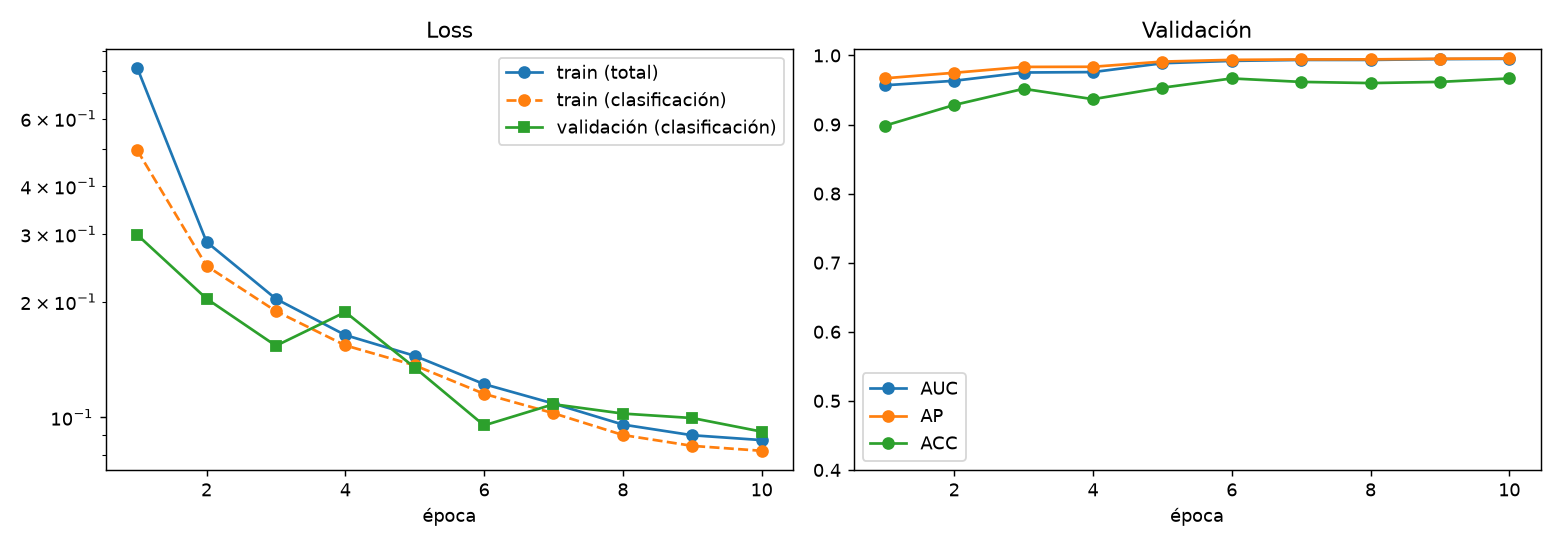
\includegraphics[width=0.85\textwidth]{curvas_it5_menos_falsas.png}
  \caption{Curvas de entrenamiento del modelo final (it5): loss (clasificación + mapa) y métricas de validación por época.}
  \label{fig:curvas}
\end{figure}

\paragraph{Desempeño del modelo final por tipo de alteración.} En prueba, el modelo final tiene AUC 0.981, AP 0.987 y recall de 93\,\% con 1\,\% de falsas alarmas (95\,\% con 5\,\%).
\begin{itemize}
  \item \textbf{Por dificultad} (recall con umbral 0.5): fácil 99\,\%, media 95\,\%, difícil 80\,\%.
  \item \textbf{Por campo:} NIT 100\,\%, total 94\,\%, fecha 89\,\%, productos 86\,\%, IVA 85\,\%.
  \item \textbf{Por técnica:} reescribir 96\,\% y copiar un dígito 63\,\%. Copiar un dígito es el punto débil: es el mismo trazo, tinta y ruido.
  \item \textbf{Por formato:} tickets y facturas carta funcionan igual (AUC 0.981 en ambos).
\end{itemize}
La figura~\ref{fig:curvas} muestra las curvas de entrenamiento. La pérdida de entrenamiento baja de forma estable y la validación se estabiliza desde la época 6. El mejor checkpoint se toma de la validación y no de la última época.

\paragraph{Problemas encontrados y cómo se resolvieron.}
\begin{enumerate}
  \item \textbf{Un primer dataset imposible.} La mitad de las alteraciones imitaban fuente, tinta, ruido y desenfoque, y a $768\times576$ eran indistinguibles. Los modelos se quedaron en AUC 0.50 (loss 0.693). Se introdujeron los niveles de dificultad, se reporta el recall por nivel y se bajó la tasa de aprendizaje de $10^{-3}$ a $3\times10^{-4}$.
  \item \textbf{Gemelas desalineadas.} El post-proceso aleatorio se sorteaba por separado para cada foto; ahora la geometría es compartida.
  \item \textbf{Validación 35 veces más lenta.} Con \texttt{channels\_last} + bf16, cuDNN construye un plan de ejecución por cada tamaño de imagen (1.2\,s contra 35\,ms por foto). Se eliminó \texttt{channels\_last} y los tamaños se redondean a múltiplos de 128.
  \item \textbf{El umbral se elegía mirando la prueba.} Esto inflaba el valor (it5: Q9,298 con $t=0.80$). Ahora se elige en validación (it5: $t=0.88$, Q9,162), y todas las iteraciones se recalcularon así.
\end{enumerate}

\paragraph{Líneas base sin deep learning.} En el mismo conjunto de prueba:
\begin{itemize}
  \item \textbf{Reglas FEL con lectura perfecta:} recall 47\,\% con 14\,\% de falsas alarmas, valor $-$Q77. Atrapan totales inflados sin ajustar el IVA, pero no fechas cambiadas ni NIT válidos de otra persona, y dan falsas alarmas en gasolineras, donde el IDP rompe la regla 12/112.
  \item \textbf{ELA:} AUC 0.507.
  \item \textbf{FacturaSegura:} recall 92\,\% con 0.7\,\% de falsas alarmas, valor Q9,162.
\end{itemize}

\section{Despliegue y experiencia de usuario}

\paragraph{Arquitectura.} FacturaSegura se despliega como una aplicación web local en Streamlit (\texttt{app/app.py}). La figura~\ref{fig:arq} muestra el flujo: el usuario sube una o varias fotos o usa la cámara, la imagen se corrige por EXIF, se procesa a resolución completa y el modelo devuelve la probabilidad y el mapa de sospecha. Con el umbral de valor se decide entre \textbf{Aprobar} o \textbf{Auditar}. Si se audita, la app muestra la foto con la zona sospechosa en rojo y un acercamiento (figura~\ref{fig:app}). Todo corre en la computadora del usuario, sin servicios externos.

\begin{figure}[h]
\centering
\begin{tikzpicture}[node distance=0.55cm, >=Stealth,
  box/.style={draw, rounded corners, fill=blue!6, align=center, font=\small, minimum height=0.95cm, text width=2.35cm},
  ok/.style={box, fill=green!12}, bad/.style={box, fill=red!10}]
  \node[box] (in) {Foto de la\\factura};
  \node[box, right=of in] (pre) {Orientación EXIF,\\máx. 1600 px,\\relleno /128};
  \node[box, right=of pre] (cnn) {EfficientNet-B0\\(fine-tuned)};
  \node[box, right=of cnn] (map) {Mapa de sospecha\\1/16 + top-8};
  \node[diamond, draw, aspect=2, fill=yellow!15, font=\small, right=0.5cm of map, inner sep=1pt] (dec) {$p\ge0.88$};
  \node[ok, above right=0.1cm and 0.5cm of dec, text width=1.6cm] (ap) {Aprobar};
  \node[bad, below right=0.1cm and 0.5cm of dec, text width=1.6cm] (au) {Auditar\\+ zona};
  \draw[->] (in) -- (pre); \draw[->] (pre) -- (cnn); \draw[->] (cnn) -- (map); \draw[->] (map) -- (dec);
  \draw[->] (dec) |- node[pos=0.25, left, font=\scriptsize]{no} (ap);
  \draw[->] (dec) |- node[pos=0.25, left, font=\scriptsize]{sí} (au);
\end{tikzpicture}
\caption{Arquitectura del sistema desplegado.}
\label{fig:arq}
\end{figure}

\begin{figure}[h]
  \centering
  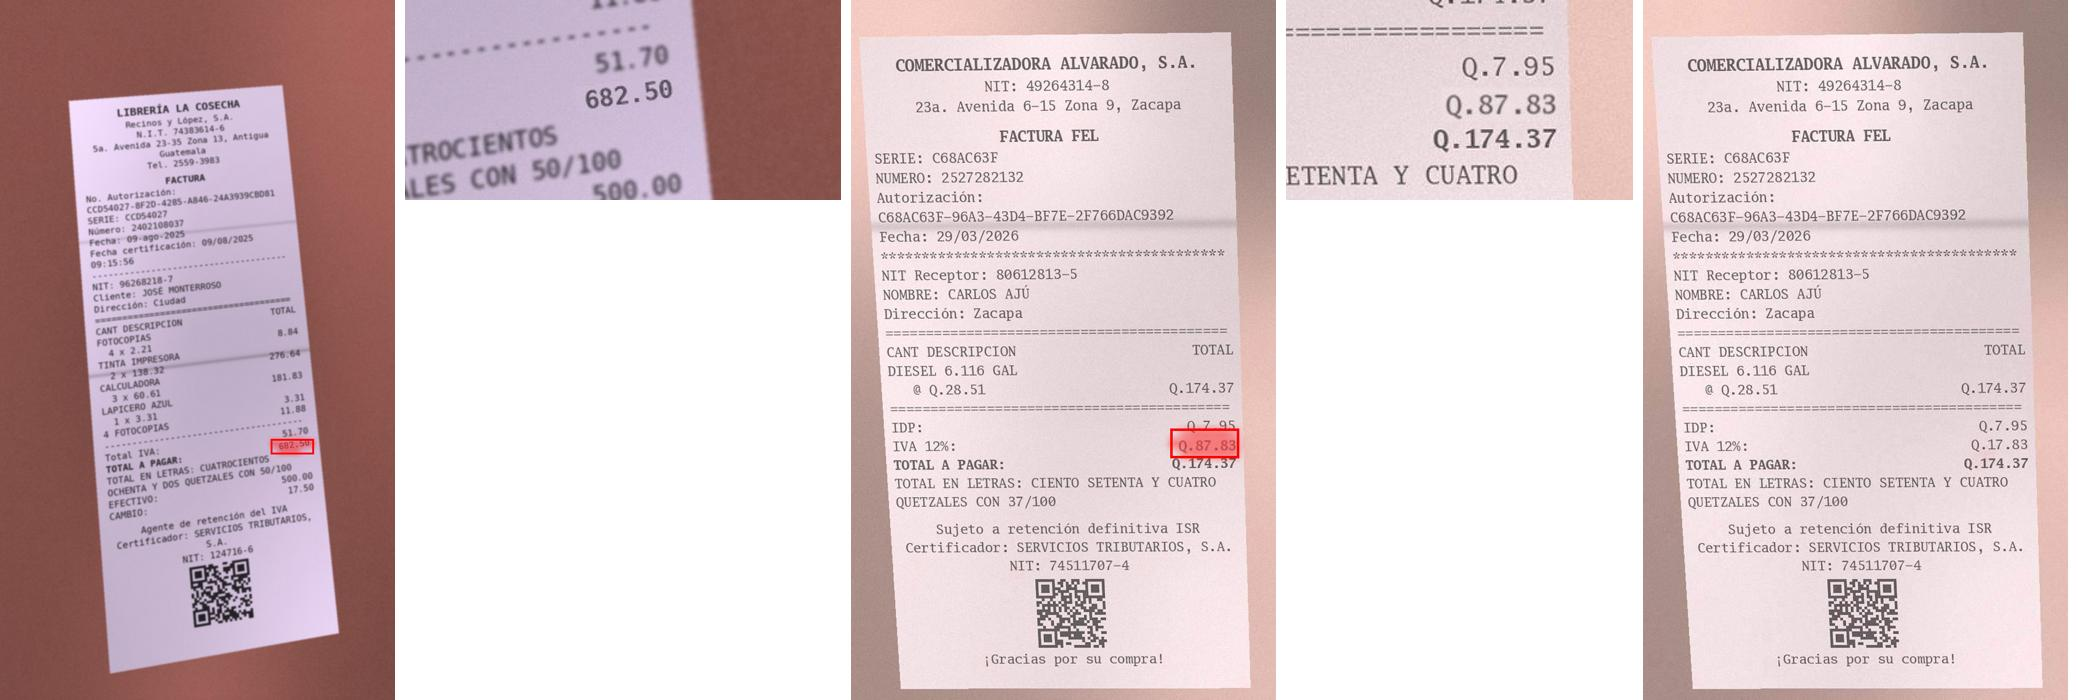
\includegraphics[width=\textwidth]{ejemplo_deteccion.jpg}
  \caption{Lo que ve el auditor. Izquierda: total cambiado de 482.50 a 682.50, marcado en rojo. Centro: IVA cambiado de 17.83 a 87.83 con la misma fuente (alteración difícil), con su acercamiento. Derecha: foto auténtica (probabilidad 8.8\,\%), aprobada sin marca.}
  \label{fig:app}
\end{figure}

\paragraph{Métricas operativas.} La latencia es de 41\,ms por foto en GPU (RTX 3070) y 0.54\,s en CPU (8 hilos), incluida la preparación de la imagen. Un auditor puede procesar un lote de cientos de facturas en minutos en cualquier laptop. El costo por predicción es prácticamente cero: no hay API ni infraestructura, y el modelo pesa 17\,MB.

\paragraph{Cómo el modelo cambia la experiencia.}
\begin{itemize}
  \item \textbf{Para el auditor:} pasa de revisar todas las facturas, o ninguna, a revisar solo 34 de cada 1,000. En cada una sabe \emph{dónde} mirar, porque el mapa acierta la zona editada en el 87\,\% de los casos. Si eso reduce el tiempo de auditoría a la mitad, el valor sube a Q9,332 (tabla~\ref{tab:sens}).
  \item \textbf{Para el empleado honesto:} la probabilidad de ser cuestionado es del 0.7\,\%.
\end{itemize}
La validación con usuarios reales (prueba de usabilidad o piloto A/B contra el proceso actual) queda como trabajo futuro.

\paragraph{Errores, casos límite e incertidumbre.}
\begin{itemize}
  \item La app rechaza archivos que no son imágenes y corrige la orientación de las fotos de celular.
  \item La probabilidad se muestra siempre. Cuando está a menos de 0.1 del umbral, aparece una advertencia de ``zona gris'' que sugiere revisar si el monto es alto.
  \item El umbral es ajustable en la interfaz, con el óptimo de valor por defecto.
  \item Cada resultado viene acompañado de un recordatorio explícito: una factura marcada no es prueba de fraude.
\end{itemize}

\paragraph{Plan de monitoreo.}
\begin{enumerate}
  \item \textbf{Deriva de entrada:} se registran la distribución de probabilidades y la tasa de facturas marcadas por semana. Un cambio brusco indica nuevos formatos de factura o nuevas apps de edición.
  \item \textbf{Retroalimentación de auditoría:} cada auditoría queda etiquetada como fraude confirmado o falsa alarma, lo que permite estimar la precisión real y la prevalencia, y recalibrar el umbral con el modelo de valor.
  \item \textbf{Auditorías aleatorias:} se audita un 1--2\,\% de facturas no marcadas para estimar el fraude que se escapa.
  \item \textbf{Reentrenamiento:} periódico con las alteraciones confirmadas, que son los ejemplos más valiosos.
\end{enumerate}

\section{Explicabilidad, ética y riesgos}

\paragraph{Explicabilidad.} Se usaron dos herramientas:
\begin{itemize}
  \item \textbf{El mapa de sospecha del propio modelo,} supervisado con máscaras. Acierta la zona editada en 87\,\% de las facturas alteradas de prueba.
  \item \textbf{Grad-CAM} sobre la última etapa del encoder. Acierta en 62\,\%; sobre el clasificador estándar (it1), solo en 25\,\%.
\end{itemize}
La ablación sin máscaras (it3b) revela algo importante: un modelo puede detectar sin mirar el lugar correcto (localización de 0\,\% con detección intacta). Sin supervisión, no hay garantía de que la decisión se apoye en la edición y no en un atajo. Por eso el modelo final mantiene las máscaras aunque no mejoren el AUC: la explicación que ve el auditor es confiable.

\paragraph{Sesgos.} El modelo funciona igual en tickets y facturas carta (AUC 0.981 en ambos) y en los seis tipos de comercio. Rinde peor en ediciones cuidadosas (copiar un dígito: 63\,\%) y en campos pequeños como el IVA (85\,\%). El costo de negocio de ese sesgo es el fraude sofisticado que se escapa, y su costo humano es el opuesto: un falso positivo recae sobre una persona concreta. Si ciertos comercios, papeles o celulares de baja calidad generaran más falsas alarmas, se acumularían sobre los mismos empleados. Esto no se puede medir con datos sintéticos y debe monitorearse con datos reales.

\paragraph{Riesgos de uso indebido y cuándo no usarlo.}
\begin{itemize}
  \item \textbf{No debe usarse para sancionar sin auditoría humana.} Es un filtro de priorización, no una prueba.
  \item \textbf{Puede ser evadido:} un defraudador que conozca el sistema podría editar el documento antes de imprimirlo, o usar técnicas que el generador no imita. Por eso conviene complementarlo con verificación contra el registro FEL de la SAT y con auditorías aleatorias.
  \item \textbf{No sirve para documentos que no sean facturas FEL fotografiadas,} ni para escaneos de muy baja resolución.
  \item \textbf{Privacidad:} las fotos contienen NIT y nombres, así que se procesan localmente y no se almacenan en servidores de terceros.
\end{itemize}

\section{Discusión y conclusiones}

\paragraph{Qué cambios movieron el valor.} Los que más aportaron fueron los de \emph{representación y operación}, no los de capacidad:
\begin{itemize}
  \item \textbf{El mapa de sospecha y la resolución completa} (+Q1,209 entre it1 e it3).
  \item \textbf{Elegir el punto de operación por valor:} un mal umbral convierte Q9,162 en una pérdida de Q19,107.
\end{itemize}
El cambio con mayor impacto en la métrica técnica (it4: AUC 0.961 $\to$ 0.984) no aumentó el valor, porque el detector se volvió más desconfiado con las facturas honestas. Solo cuando se corrigió ese efecto (it5) la mejora técnica se tradujo en un modelo más robusto con igual o más valor.

\paragraph{Rendimientos decrecientes.} El modelo final detiene el 94\,\% del fraude en quetzales. De los ${\sim}$Q1,130 por cada 1,000 facturas que lo separan del fraude total:
\begin{itemize}
  \item Q662 son fraude no detectado;
  \item Q275 es el costo inevitable de auditar los fraudes reales;
  \item ${\sim}$Q190 vienen de las falsas alarmas.
\end{itemize}
Incluso un modelo perfecto ganaría como mucho ${\sim}$Q800 más, una cifra del mismo orden que el ruido de medición con 300 facturas por clase. Desde aquí, seguir mejorando el modelo deja de valer la pena. Una regla de decisión que consideraba el monto reclamado tampoco mejoró el ahorro. Las palancas que quedan son de producto: auditorías más rápidas gracias al mapa, verificación automática contra la SAT antes de contactar al empleado (que eliminaría casi toda la fricción) y una mejor estimación de la prevalencia real.

\paragraph{Complejidad, costo y valor.} El modelo final usa la arquitectura más pequeña probada (EfficientNet-B0, 17\,MB, 0.5\,s por foto en CPU), cuesta menos de una hora de GPU de laptop y tiene un costo de operación prácticamente nulo. Para una empresa que procesa 1,000 facturas de reembolso al mes, el ahorro estimado es del orden de Q9,000 mensuales con los supuestos base, por lo que la propuesta es viable incluso con supuestos bastante más pesimistas.

\paragraph{Limitaciones.}
\begin{itemize}
  \item \textbf{Todos los resultados son sintéticos.} El desempeño con fotos reales editadas con apps comunes no se ha medido, y es de esperar una caída si esas apps usan técnicas que el generador no imita.
  \item \textbf{Los supuestos de valor son estimaciones,} en particular la prevalencia.
  \item \textbf{El conjunto de prueba es pequeño} (300 por clase) para distinguir diferencias menores a ${\sim}$Q300.
\end{itemize}

\paragraph{Viabilidad y siguientes pasos.}
\begin{enumerate}
  \item Recolectar fotos reales de facturas auténticas y editadas para medir y ajustar el modelo.
  \item Ampliar validación y prueba a ${\sim}$1,000 pares, para poder distinguir mejoras pequeñas.
  \item Agregar al generador nuevas técnicas de edición observadas en la práctica.
  \item Hacer un piloto con un área contable real para medir tiempos de auditoría y prevalencia.
  \item Integrar la verificación contra el registro FEL.
\end{enumerate}

\section{Repositorio}

El código completo está en \url{https://github.com/anthonylouschwank/ProyectoFInal-DL}. Incluye:
\begin{itemize}
  \item la generación de datos (\texttt{src/synth\_fel.py}, \texttt{src/tamper.py}, \texttt{src/build\_dataset.py});
  \item el modelo y el entrenamiento (\texttt{src/model.py}, \texttt{train/train.py});
  \item la evaluación, el modelo de valor y las líneas base (\texttt{eval/evaluate.py});
  \item la aplicación (\texttt{app/app.py});
  \item pruebas automáticas (\texttt{tests/}).
\end{itemize}
El \texttt{README.md} explica cómo instalar, ejecutar y reproducir las métricas. \texttt{RESULTADOS.md} detalla todas las iteraciones, y \texttt{ITERACIONES.md} documenta la configuración y el protocolo para continuar el trabajo.

\end{document}
